\documentclass{standalone}
\usepackage{tikz}
\usetikzlibrary{arrows.meta}

\begin{document}
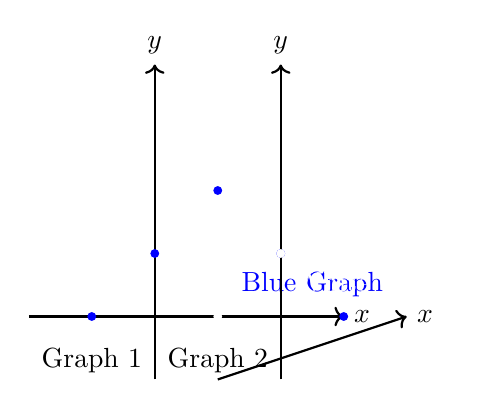
\begin{tikzpicture}[scale=0.8]

% Background
\fill[white] (-2,-1) rectangle (5,4);

% Axes for the first graph
\draw[->,thick] (-2,0) -- (3,0) node[right] {$x$};
\draw[->,thick] (0,-1) -- (0,4) node[above] {$y$};

% Data points for the first graph
\foreach \x/\y in {-1/1, 0/2, 1/3, 2/2, 3/1} {
    \fill[blue] (\x,-1+\y) circle (2pt);
}

% Labels for the first graph
\node at (-1,-0.7) {Graph 1};
\node at (2.5,0.5) {\textcolor{blue}{Blue Graph}};

% Axes for the second graph
\draw[->,thick] (1,-1) -- (4,0) node[right] {$x$};
\draw[->,thick] (2,-1) -- (2,4) node[above] {$y$};

% Data points for the second graph
\foreach \x/\y in {0/1, 1/2, 2/3, 3/2, 4/1} {
    \fill[white] (\x+1,-1+\y) circle (2pt);
}

% Labels for the second graph
\node at (1,-0.7) {Graph 2};
\node at (3.5,0.5) {\textcolor{white}{White Graph}};

\end{tikzpicture}
\end{document}